\section{Data}
\subsection{Speeches}
For this study I have collected 2486 speeches covering a time period from 2003 to 2021 (see Table \ref{tab:dates}). Speeches' data set was downloaded from the ECB website\footnote{\href{https://www.ecb.europa.eu/press/key/date/html/index.en.html}{See speeches data set here}}. Speeches are divided according to a policy makers role - President, Vice-President and the remaining executive Board Members. All the speeches given by the ECB's Presidents since the ECB's establishment is recorded under the President category, etc. Table %\ref{tab:speechspeak} 
provides a summary of speakers that my speech data comprises.

\begin{table} [!ht]
\centering
\caption{Sample Size: Dates}
\label{tab:dates}
\begin{adjustbox}{width=0.5\textwidth}
\begin{tabular}[t]{lll}
\toprule
Indicator & Min date & Max date\\
\midrule
Interest Rates & 2004-09-09 & 2021-07-01\\
Credit Spreads & 2012-08-03 & 2021-07-19\\
Inflation Expectations & 2010-07-22 & 2021-07-19\\
Euro Stoxx 50 & 1997-01-06 & 2021-07-28\\
Speeches & 2003-03-03 & 2021-05-29\\
\addlinespace
 &  & \\
Eonia & 2003-01-03 & 2021-07-01\\
CESI & 2003-01-03 & 2021-07-01\\
 &  & \\
Financial Crisis dummy & 2007-06-01 & 2009-12-31\\
\addlinespace
Covid-19 Crisis dummy & 2020-03-01 & 2021-07-01\\
\bottomrule
\end{tabular}
\end{adjustbox}
\end{table}

%\begin{table}[!ht]
    \centering
    \caption{Speaker Speeches Descriptives}
    \resizebox{\textwidth}{!}{\begin{tabular}[h]{cccccc}
    \toprule
    role & n$^o$ of speeches (role) & speakers & n$^o$ of speeches (speaker) & min date & max date\\
    \midrule
     &  & Benoît Cœuré & 191 & 2012-02-06 & 2019-12-18\\
    \cmidrule{3-6}
     &  & Eugenio Domingo Solans & 76 & 1998-06-26 & 2004-04-23\\
    \cmidrule{3-6}
     &  & Fabio Panetta & 21 & 2020-02-18 & 2021-05-19\\
    \cmidrule{3-6}
     &  & Frank Elderson & 2 & 2021-01-25 & 2021-04-29\\
    \cmidrule{3-6}
     &  & Gertrude Tumpel-Gugerell & 159 & 2003-06-30 & 2011-05-23\\
    \cmidrule{3-6}
     &  & Isabel Schnabel & 30 & 2020-01-09 & 2021-05-27\\
    \cmidrule{3-6}
     &  & Jörg Asmussen & 51 & 2012-03-27 & 2013-12-12\\
    \cmidrule{3-6}
     &  & José Manuel González-Páramo & 119 & 2004-11-11 & 2012-05-18\\
    \cmidrule{3-6}
     &  & Jürgen Stark & 88 & 2006-07-17 & 2011-12-02\\
    \cmidrule{3-6}
     &  & Lorenzo Bini Smaghi & 119 & 2005-10-10 & 2011-12-16\\
    \cmidrule{3-6}
     &  & Otmar Issing & 100 & 1998-07-02 & 2006-05-22\\
    \cmidrule{3-6}
     &  & Peter Praet & 129 & 2011-06-16 & 2019-05-15\\
    \cmidrule{3-6}
     &  & Philip R. Lane & 35 & 2019-07-01 & 2021-05-25\\
    \cmidrule{3-6}
     &  & Sabine Lautenschläger & 85 & 2014-02-03 & 2019-10-30\\
    \cmidrule{3-6}
     &  & Sirkka Hämäläinen & 43 & 1998-10-26 & 2003-04-28\\
    \cmidrule{3-6}
     &  & Tommaso Padoa-Schioppa & 47 & 1998-09-03 & 2004-11-03\\
    \cmidrule{3-6}
    \multirow{-17}{*}{\centering\arraybackslash Board Members} & \multirow{-17}{*}{\centering\arraybackslash 1456} & Yves Mersch & 161 & 2013-02-27 & 2020-11-04\\
    \cmidrule{1-6}
     &  & Alexandre Lamfalussy & 7 & 1997-02-07 & 1997-06-30\\
    \cmidrule{3-6}
     &  & Christine Lagarde & 31 & 2019-11-04 & 2021-05-06\\
    \cmidrule{3-6}
     &  & Jean-Claude Trichet & 329 & 2003-11-20 & 2011-10-24\\
    \cmidrule{3-6}
     &  & Mario Draghi & 186 & 2011-11-18 & 2019-10-28\\
    \cmidrule{3-6}
    \multirow{-5}{*}{\centering\arraybackslash President} & \multirow{-5}{*}{\centering\arraybackslash 710} & Willem F. Duisenberg & 157 & 1997-06-30 & 2003-10-29\\
    \cmidrule{1-6}
     &  & Christian Noyer & 51 & 1998-10-01 & 2002-04-23\\
    \cmidrule{3-6}
     &  & Lucas Papademos & 87 & 2003-03-07 & 2010-05-31\\
    \cmidrule{3-6}
     &  & Luis de Guindos & 56 & 2018-06-26 & 2021-05-27\\
    \cmidrule{3-6}
    \multirow{-4}{*}{\centering\arraybackslash Vice-President} & \multirow{-4}{*}{\centering\arraybackslash 320} & Vítor Constâncio & 126 & 2010-07-09 & 2018-05-17\\
    \bottomrule
    \end{tabular}
    \label{tab:speechtable_descriptives}
    \begin{tablenotes}
    \item{\textit{Note.} "min date" and "max date" indicates a time when a particular speaker gave the first and the last speech respectively.}
    \end{tablenotes}
    \end{table}
    
%%%%%%%%%%%%%%%%%%%%%%%%%%%%%%%%%%%%%%%%%%%%%%%%%%%%%%%%%%%%%%%%%%%%%%
\subsection{Asset Prices}
I look at bond yields, credit spread, equity returns, and inflation expectations for the Euro area. For these asset prices, I take daily data, which is necessary for matching these with the speech data. For the bond yields, I take triple AAA-rated Euro area government bonds which are readily available on the ECB’s website\footnote{\href{https://www.ecb.europa.eu/stats/financial_markets_and_interest_rates/euro_area_yield_curves/html/index.en.html}{See Euro area yield data here}} at the daily frequencies. The composition in terms of specific Euro area countries varies accordingly with the updated ratings by Fitch (see Table \ref{tab:ratings} in Appendix \ref{ap:data}). My yield data spans from 2004 to 2021 (see Table \ref{tab:dates}) and includes bonds with maturities of 3 months, 1-, 2-, 5-, 7-, 10-, 20-, 30-years.


The Euro area credit spread is the difference between Italian and German sovereign bonds. I retrieve Italian and German government bond yields from the Refinitiv database. However, due to many missing observations I only have credit spread data spanning from 2012 to 2021 (see Table \ref{tab:dates}), with maturities of 3 months, 1-, 2-, 5-, 7-, 10-, 15-, 20- and 30-years.



For the equity returns, I use the Euro Stoxx 50 index returns covering the period from 1997 to 2021 (see Table \ref{tab:dates}). This data is obtained from FactSet.


I did not have access to the daily inflation expectations for the Euro area. For this reason, I take German 5-year breakeven inflation as a proxy for the Euro area’s inflation expectations. The German 5-year breakeven inflation is constructed as the difference between the 5-year nominal bond and an inflation-linked bond of the same maturity and is retrieved from Refinitiv. 5-year maturity is chosen due to its data completeness. My final inflation expectations data spans from 2010 to 2021 (see Table \ref{tab:dates}).


%\begin{figure}
%	\centering
 	%\fbox{\rule[-.5cm]{4cm}{4cm} \rule[-.5cm]{4cm}{0cm}}
% 	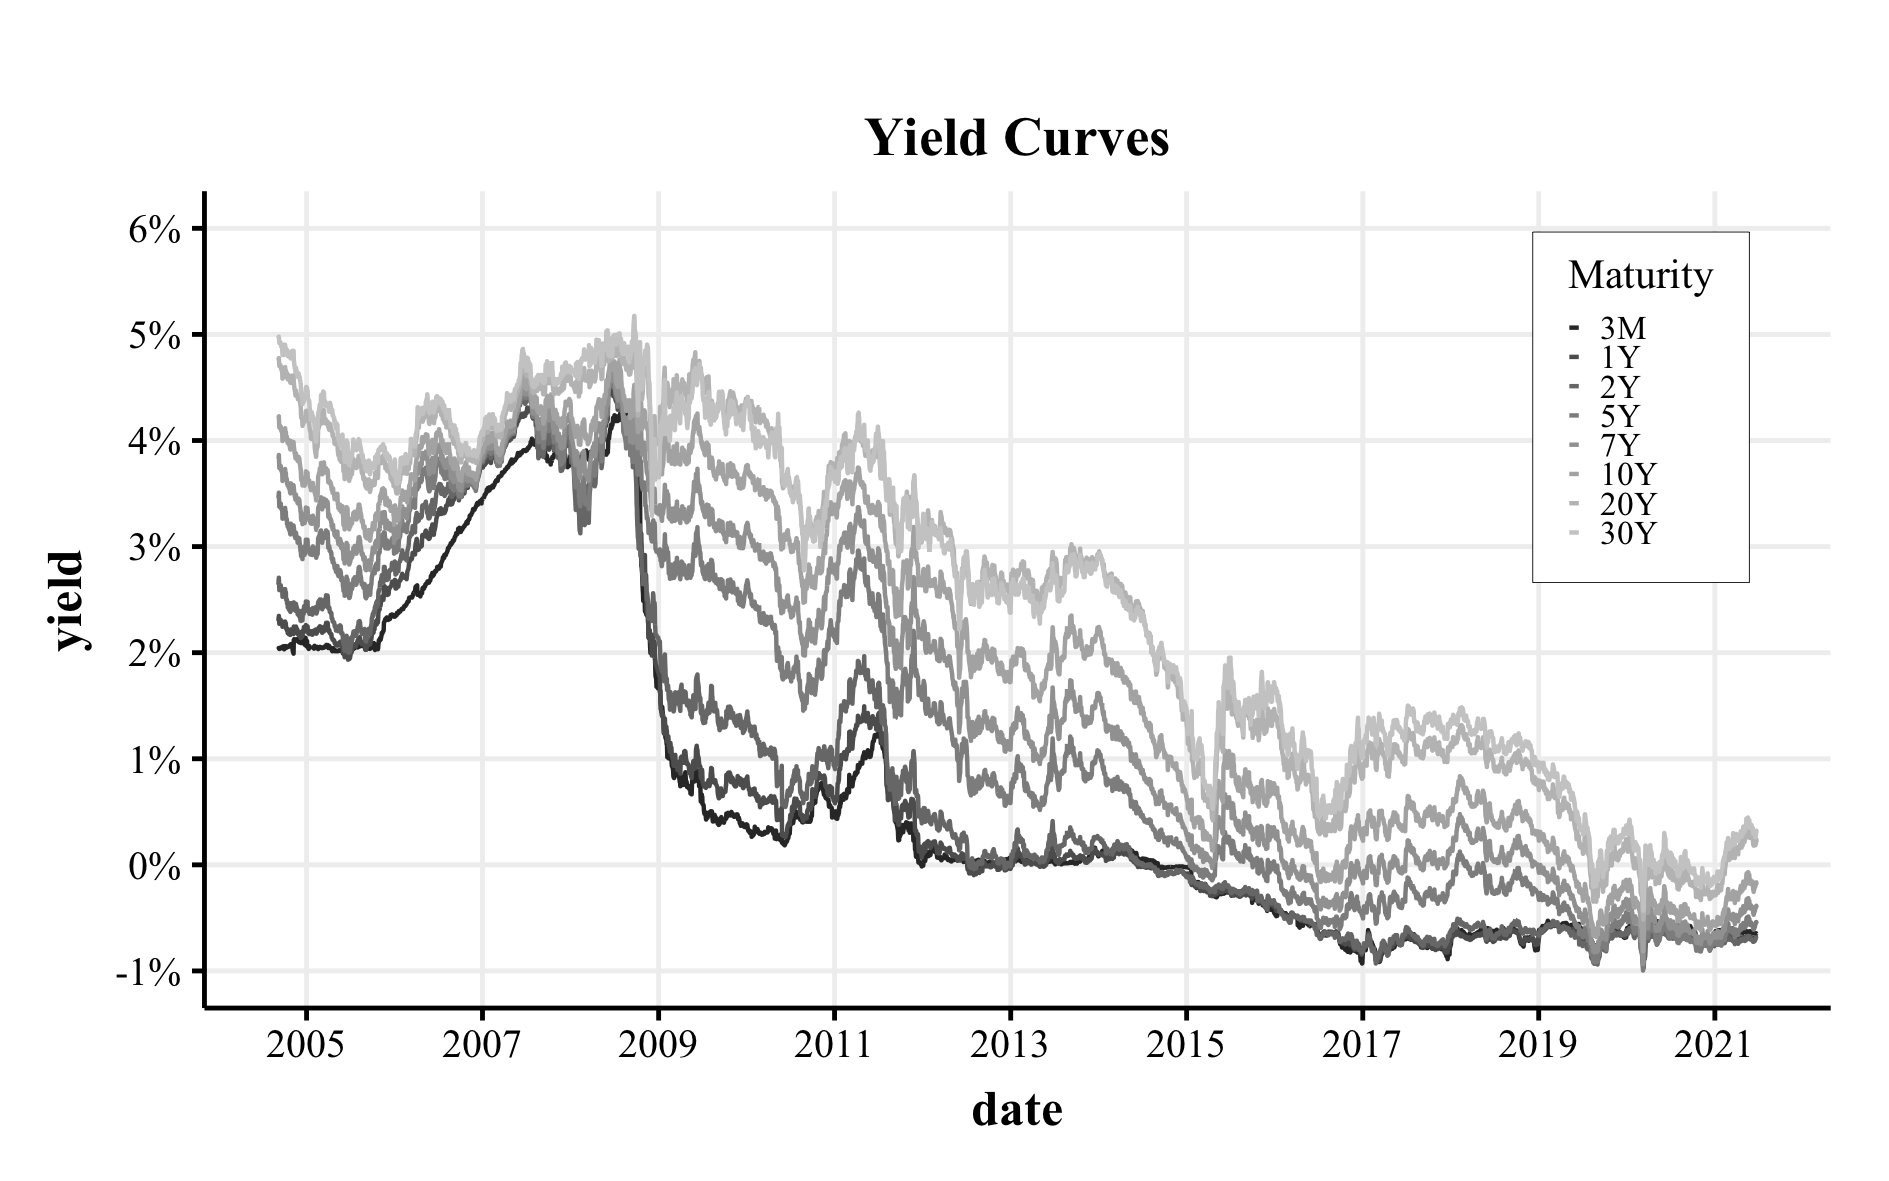
\includegraphics[width=0.7\textwidth]{Figures/yield_curves.png}
% 	\caption{Eurozone yield curves (spot rates) with maturities of 3 months, 1-, 2-, 5-, 7-, 10-, 20-, 30-years; daily frequency; September 2004 - June 2021; consisting of government  nominal bonds whose rating is triple A. (European Central Bank)}
% 	\label{fig:fig1}
% \end{figure}
 
%%%%%%%%%%%%%%%%%%%%%%%%%%%%%%%%%%%%%%%%%%%%%%%%%%%%%%%%%%%%%%%%%%%%%%

\subsection{Control Variables}
To isolate the effect of the speeches, I control for the day-of-the-week effects, the monetary policy shocks, and the surprises of the various macroeconomic news as recommended by the literature (see, e.g., \cite{ehrmann2007,rozkrut2007}). I use the change in the Eonia rate as a measure of monetary policy shocks. I obtain daily data for the Eonia rate from the ECB website covering the period from 2003 to 2021 (see Table \ref{tab:dates}). To control for the macroeconomic surprises, I use the Euro area Citigroup Economic Surprise Index (CESI), which is the weighted moving average of all macroeconomic news surprises relevant to the Euro area. CESI is compiled by Bloomberg and a positive (negative) reading of the CESI suggests that economic news have on balance beaten (fall back) consensus expectations. I gathered CESI from Refinitiv. My Euro area CESI data covers the period from 2003 to 2021 (see Table \ref{tab:dates}).
